\documentclass[a4paper,12pt]{report}
\usepackage[french]{babel}
\usepackage[utf8]{inputenc}
\usepackage[T1]{fontenc}
\usepackage[a4paper, top=2cm, bottom=2.5cm, left=2cm, right=2cm]{geometry}


\usepackage{graphicx}
\usepackage{caption}
\usepackage{subcaption}
\usepackage{lmodern}
\usepackage{parskip}
\usepackage{microtype}
\usepackage{enumitem}
\usepackage{booktabs}
\usepackage{tabularx}
\usepackage{booktabs}
\usepackage{array}
\usepackage[ruled,vlined]{algorithm2e}


\usepackage{hyperref}
\hypersetup{
    colorlinks=true,
    linkcolor= black,
    filecolor=magenta,      
    urlcolor=cyan,
    pdftitle={Overleaf Example},
    pdfpagemode=FullScreen,
}

\begin{document}
\begin{titlepage}
    \centering
    \vspace*{0.2cm} 
    

    
    % Optional logo
    
\includegraphics[width=0.5\textwidth]{upc.jpg}\par
    \vspace{1cm}

    
     \textbf{\Large Cahier de conception} \\[1em]
    \textquotedblleft \textsc{Projet de programmation} \textquotedblright \\[1em]
    \textbf{\large Sujet} \\[1em]
    \rule{\textwidth}{0.4pt} \\[1em]
    \textbf{\LARGE
    Développement d’un système de recommandation basique } \\[1em]
    \rule{\textwidth}{0.4pt}

    \vspace{1.8cm}
    
    
    

\noindent
\begin{minipage}[t]{0.45\textwidth}
    \textbf{\large Réalisé par:} \\[1em]
    Dihya MEGHERFI \\
    Dina BOUDERKA \\
    Lilia JESOVER--ENGEL \\
    Adriana NGANZU NDAYIDI \\
    
\end{minipage}
\hfill
\begin{minipage}[t]{0.45\textwidth}
    \raggedleft
    \textbf{\large Encadré par:} \\[1em]
    M Enzo BONNEAU
\end{minipage}

    \vspace{1.2cm}
    
 \rule{\textwidth}{0.4pt} \\[1em]
    \textbf{\LARGE
    Année: 2025/2026}\\

    \vfill
\end{titlepage}


\newpage
\tableofcontents
\newpage
\listoftables
\listoffigures
\chapter{Introduction}
Le livrable de conception détaillée s'inscrit dans le cadre du projet de développement d'un système de recommandation de films. Ce document présente l'architecture prévue du système, la description des principaux composants et modules, ainsi que la structure des données et des fonctionnalités attendues. Il a pour but de servir de référence avant le développement, afin de guider l'implémentation future et d'assurer la cohérence avec le cahier des charges.

La démarche adoptée repose sur une analyse des spécifications fonctionnelles du projet. À partir de ces exigences, les différentes parties du système sont décrites afin de préciser leur rôle et leur fonctionnement au sein de l'application. Cette étape permet de structurer le développement futur et d'assurer une cohérence entre les besoins identifiés et la solution proposée.

\section{Objectifs et méthodes}
L'objectif principal de ce document est de détailler la conception du système de recommandation de films avant sa phase de développement. Il vise à présenter l'organisation générale de l'application, les différents composants du système ainsi que les fonctionnalités prévues pour répondre aux besoins définis dans le cahier des charges.

\section{Documents de référence}
Les documents ayant servi de base à l’élaboration du cahier de conception sont :

\begin{itemize}
    \item Le cahier des charges du projet.
    \item Le cahier de recette du projet.
    \item Les maquettes de l’interface utilisateur.
    \item La documentation du jeu de données utilisé : \texttt{The Movies Dataset}.
    \item La documentation de l’outil d’hébergement : \texttt{AWS}.
\end{itemize}

\chapter{Guide de lecture}
Ce document présente la conception détaillée du système de recommandation de films. Il est destiné à plusieurs types de lecteurs. 
\section{Maîtrise d'œuvre}

La maîtrise d'œuvre est constituée des quatre étudiantes responsables de la 
conception et du développement du système. Le rôle de chef de projet est 
assuré à tour de rôle par les membres de l'équipe.

\begin{itemize}
\item Dihya MEGHERFI
\item Dina BOUDERKA
\item Lilia JESOVER-ENGEL
\item Adriana NGANZU NDAYIDI
\end{itemize}

\subsubsection{Responsable}

La personne assurant le rôle de responsable organise les réunions de suivi, 
coordonne les activités de l’équipe, répartit les tâches et veille au respect 
du planning ainsi qu’à l’avancement global du projet.

\subsubsection{Personnel technique}

L’ensemble des membres de l’équipe participe aux activités techniques du projet, 
notamment :

\begin{itemize}
\item Conception de l’architecture cloud AWS (Amplify, Cognito, DynamoDB, AppSync, Lambda)
\item Développement du backend Python (Lambda de recommandation)
\item Développement du frontend en Vue.js
\item Traitement du dataset de films et implémentation de l’algorithme de recommandation
\item Réalisation des tests et intégration du système
\item Rédaction de la documentation technique
\end{itemize}

\section{Maîtrise d'ouvrage}

La maîtrise d'ouvrage est représentée par l’UFR Mathématiques et Informatique 
de l’Université Paris Cité, ainsi que par l’encadrant pédagogique, 
M. Enzo Bonneau.

La maîtrise d’ouvrage est chargée de définir les objectifs du projet, de valider 
les fonctionnalités développées, d’évaluer la conformité du système au cahier 
des charges et d’approuver le produit final.

\chapter{Concepts de base}
\begin{itemize}
    \item \textbf{Architecture :} L’architecture d’un système informatique désigne l’organisation générale de ses composants logiciels et matériels ainsi que les interactions entre eux. Elle décrit comment les différentes parties du système sont structurées et collaborent pour assurer le fonctionnement global de l’application.
        \item \textbf{Interface web :} Interface accessible via un navigateur permettant à l’utilisateur d’interagir avec le système. Le
système inclut une interface permettant :
\begin{itemize}
    \item De consulter les recommandations de films générées.
    \item De noter des œuvres.
    \item De rechercher des films.
\end{itemize}
Les tests vérifieront la cohérence entre les actions de l’utilisateur et les résultats affichés.
    \item \textbf{Système de recommandation :} Un système de recommandation est un outil informatique permettant de proposer des éléments à un utilisateur en prédisant ses préférences, en se basant sur les notes qu’il attribue à d’autres éléments ainsi que les informations associées à ces derniers.

    \item \textbf{Jeu de données (dataset) :}
Le modèle s’appuie sur un jeu de données qui est un ensemble structuré d’informations. Dans
ce projet, il contient des films avec leurs caractéristiques (titre, genre, note moyenne, réalisateur,
année de sortie) ainsi que les notes attribuées par des utilisateurs.

\item \textbf{Base de données :} Une base de données est un ensemble organisé de données stockées sous forme de plusieurs jeux de données.
    \item \textbf{Authentification :} Une méthode chiffrée qui permet aux appareils et aux personnes de s'identifier auprès d'autres appareils et systèmes.

\end{itemize}

\chapter{Conception générale}
Ce chapitre a pour but de présenter la structure générale de l'application Recomodo. On y trouvera ses principales fonctionnalités, son architecture et certaines interactions entre les différents services.
\section{Grands domaines fonctionnels}
\label{df}
L'application Recomodo se divise en plusieurs domaines fonctionnels :
\begin{table}[h]
        \centering
        \begin{tabular}{@{}ll@{}}
            \toprule
            \textbf{Domaine Fonctionnel} & \textbf{Description}\\
            \midrule
            \textbf{Interface web} & Affiche les informations, récupère les actions de l'utilisateur\\
            \textbf{Connexion et préférences utilisateur} & Inscription, connexion, gestion de profil\\
            \textbf{Business Logic/Middleware} & Coordonne les échanges entre les différents services\\
            \textbf{Système de recommandation} & Propose une liste de films recommandés pertinente\\            \textbf{Base de données} & Données utilisateurs et données des films\\
            \bottomrule
        \end{tabular}
\end{table}
\newpage

\section{Architecture de l'application}
\label{archi}
\subsection{Paradigme de programmation utilisé}
L'application repose sur le paradigme de la programmation impérative. Le backend sera constitué de micro-services.

\subsection{Principaux composants logiciels}
\begin{itemize}
    \item \textbf{AWS Amplify} : AWS Amplify est une plateforme de développement qui facilite le déploiement et l’intégration d’applications web avec les services AWS. Dans ce projet, elle est utilisée pour héberger l’interface web et simplifier la connexion avec les services backend.
    \item \textbf{AWS Cognito} : AWS Cognito est un service d’authentification et de gestion des utilisateurs. Il permet de gérer l’inscription, la connexion et la vérification des utilisateurs de manière sécurisée.
    \item \textbf{API Gateway} : L’API Gateway constitue l’interface de communication entre l’application web et les services backend. Elle permet de transmettre les requêtes envoyées par l'interface utilisateur aux bons services dans le backend et de renvoyer les réponses correspondantes. 
    \item \textbf{AWS Lambda} : AWS Lambda est un service de calcul sans serveur permettant d’exécuter du code en réponse à des événements. Dans ce projet, les fonctions Lambda implémentent la logique métier et certaines parties du système de recommandation.  
    \item \textbf{DynamoDB} : DynamoDB est une base NoSQL de données proposée par AWS. Elle nous servira à stocker les informations utilisateur, ainsi que les informations sur les films.
    \item \textbf{AWS S3} : AWS S3 est un service de stockage d’objets utilisé pour conserver les affiches des films, des documents ou d’autres ressources associées aux éléments recommandés.
    \item \textbf{Python} : Le système de recommandation ainsi que d'autres parties du backend seront implémentées en python. Pour le système de recommandation les librairies principales sont \texttt{Pandas} et \texttt{Sickit-learn}.
    \item \textbf{Vue} : Vue est un framework \texttt{JavaScript} que nous allons utiliser pour développer l'interface utilisateur interactive et dynamique. Nous utiliserons l'extension \texttt{TypeScript} de \texttt{JavaScript}.
    \item \textbf{Node.js} : Node.js est un environnement d’exécution \texttt{JavaScript} côté serveur. Il permet d'utiliser le même langage pour le frontend et le backend. Nous utiliserons l'extension de \texttt{JavaScript} : \texttt{TypeScript} pour ce projet.
\end{itemize}

\begin{figure}[h]
    \centering
    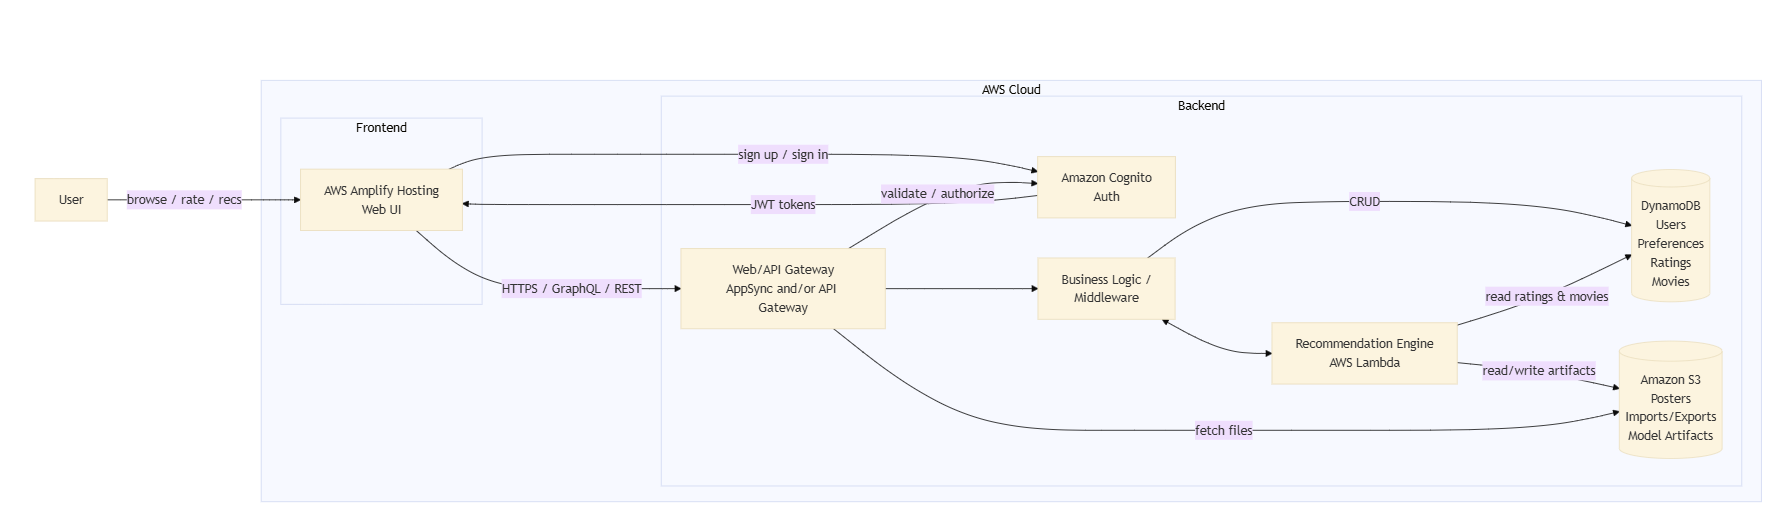
\includegraphics[width=1\textwidth]{architecture_mermaid.png}
    \caption{Architecture}
\end{figure}

\newpage

\section{Diagrammes UML}
\label{UML}
Les différentes interactions entre les composants sont modélisées à l'aide des 
diagrammes UML : 
\begin{itemize}
    \item \textbf{Diagramme de cas d'utilisation} :
    \begin{figure}[h]
        \centering
        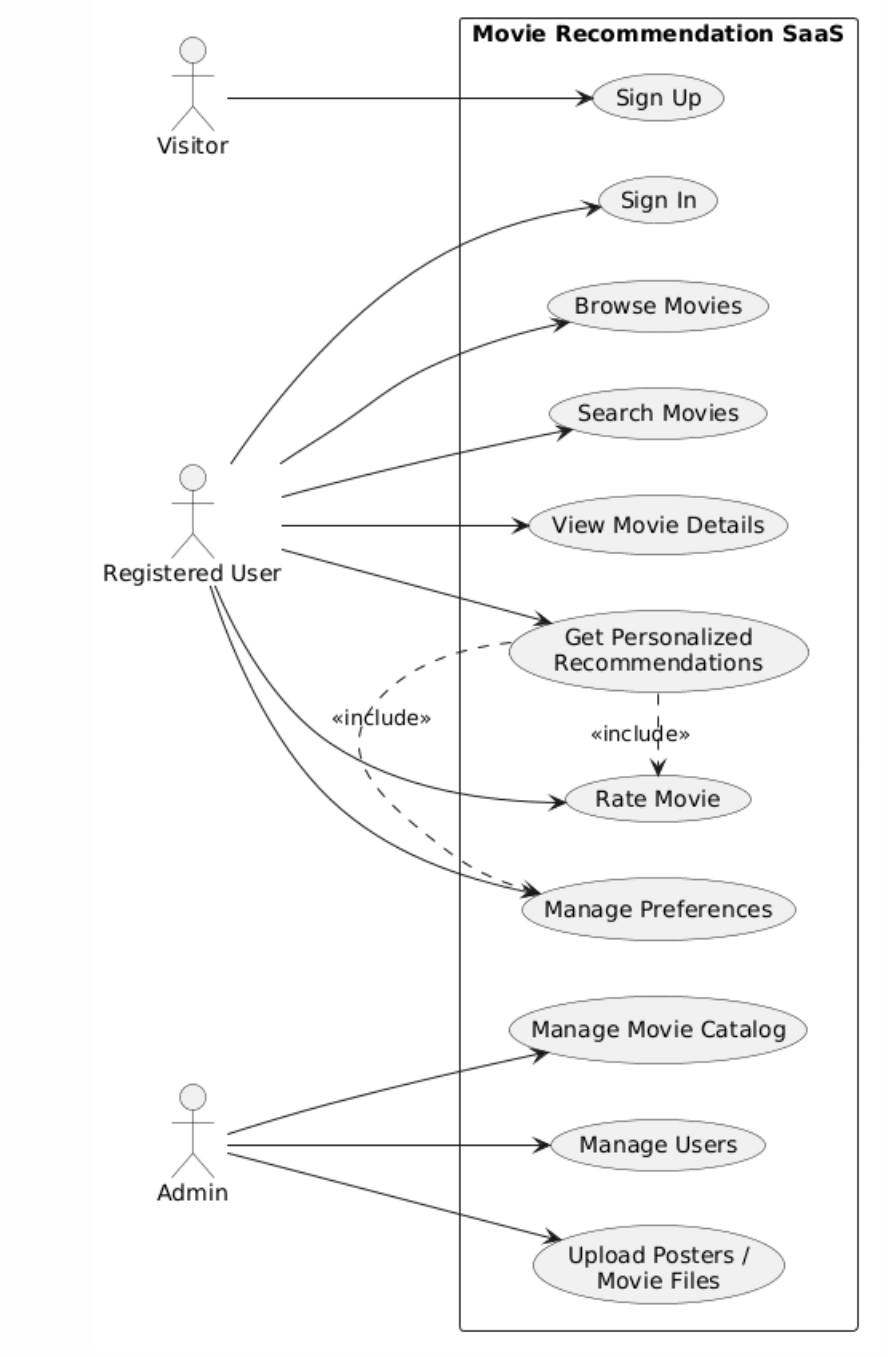
\includegraphics[width=0.7\textwidth]{use_case.png}
        \caption{Diagramme de cas d'utilisation}
    \end{figure}
    \newpage
    
    \item \textbf{Diagrammes de séquences}
    \begin{figure}[h]
        \centering
        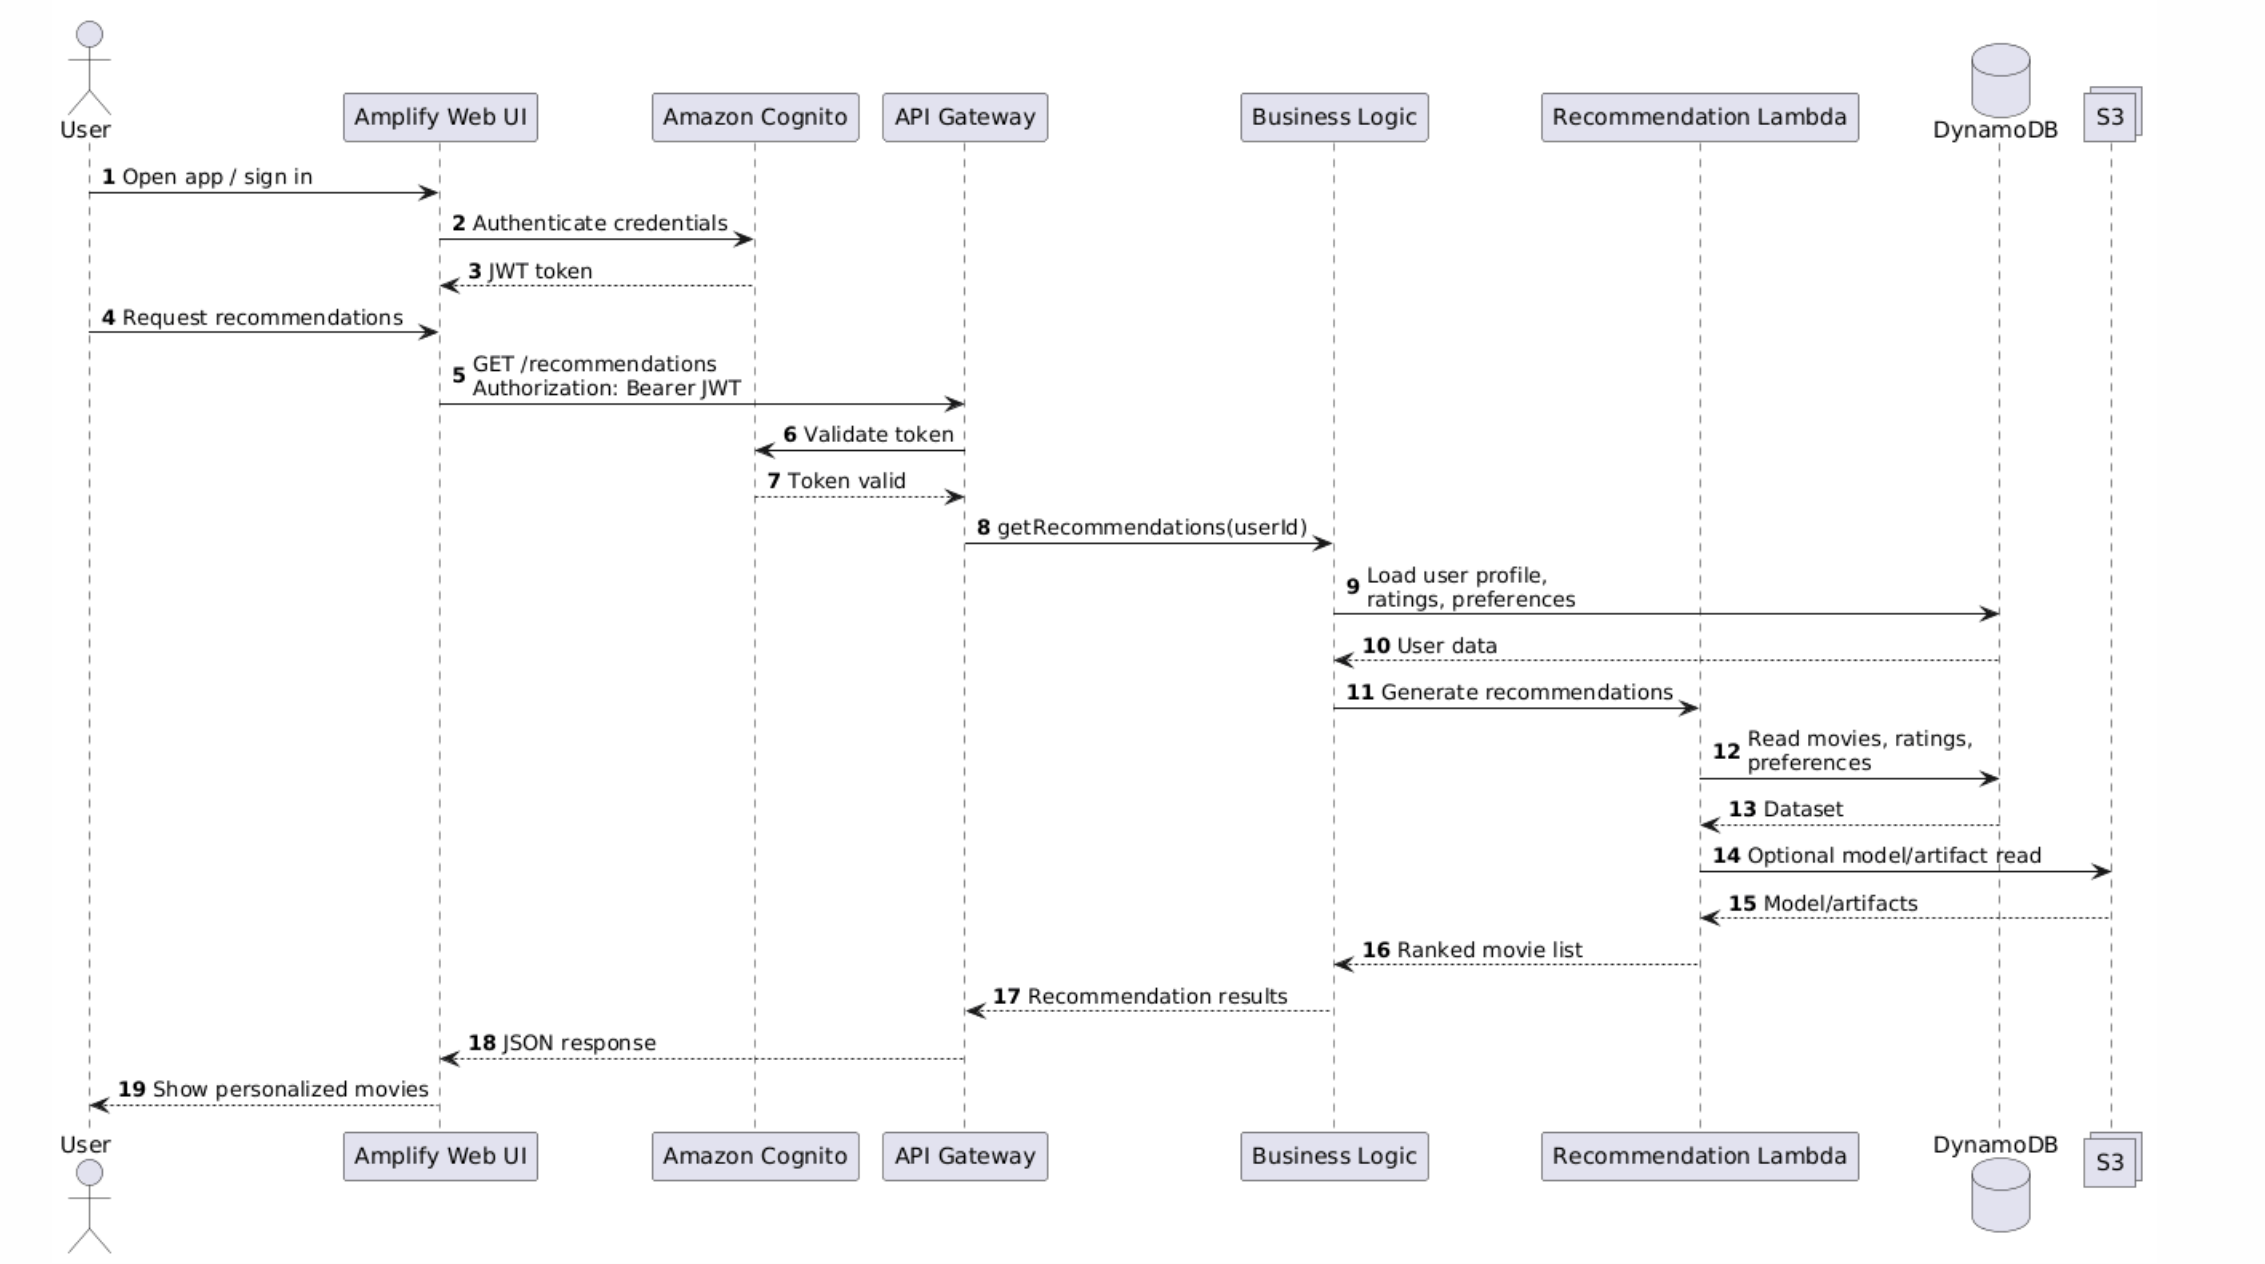
\includegraphics[width=1\textwidth]{diagramme_seq_reco.png}
        \caption{Diagramme de séquences de demande de recommandation}
    \end{figure}

    \begin{figure}[h]
        \centering
        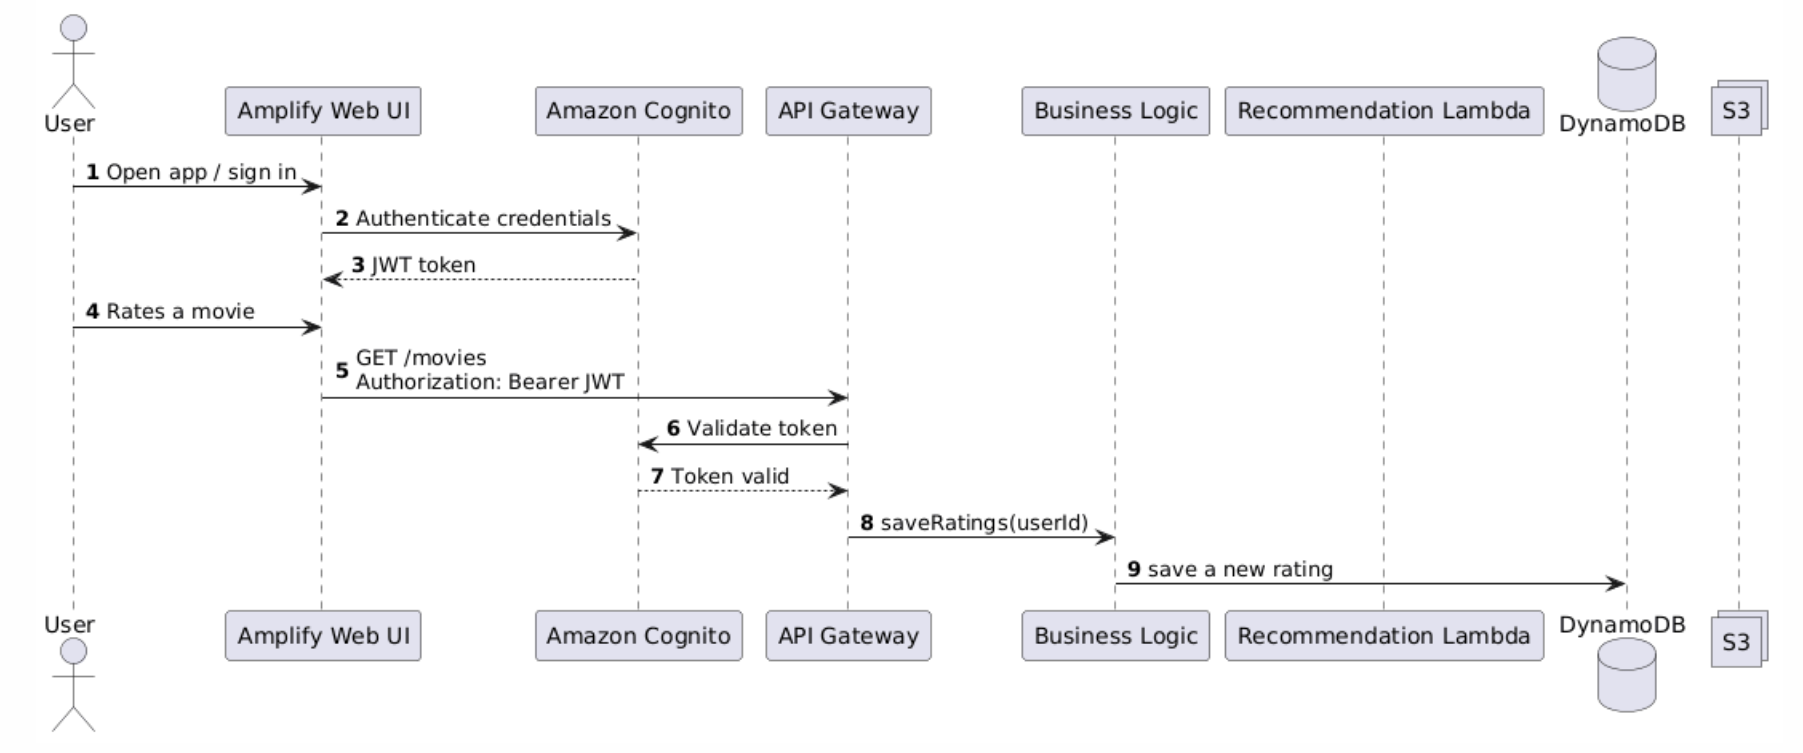
\includegraphics[width=1\textwidth]{diagramme_seq_rate.png}
        \caption{Diagramme de séquences de notation}
    \end{figure}
    \newpage
    \begin{figure}[h]
        \centering
        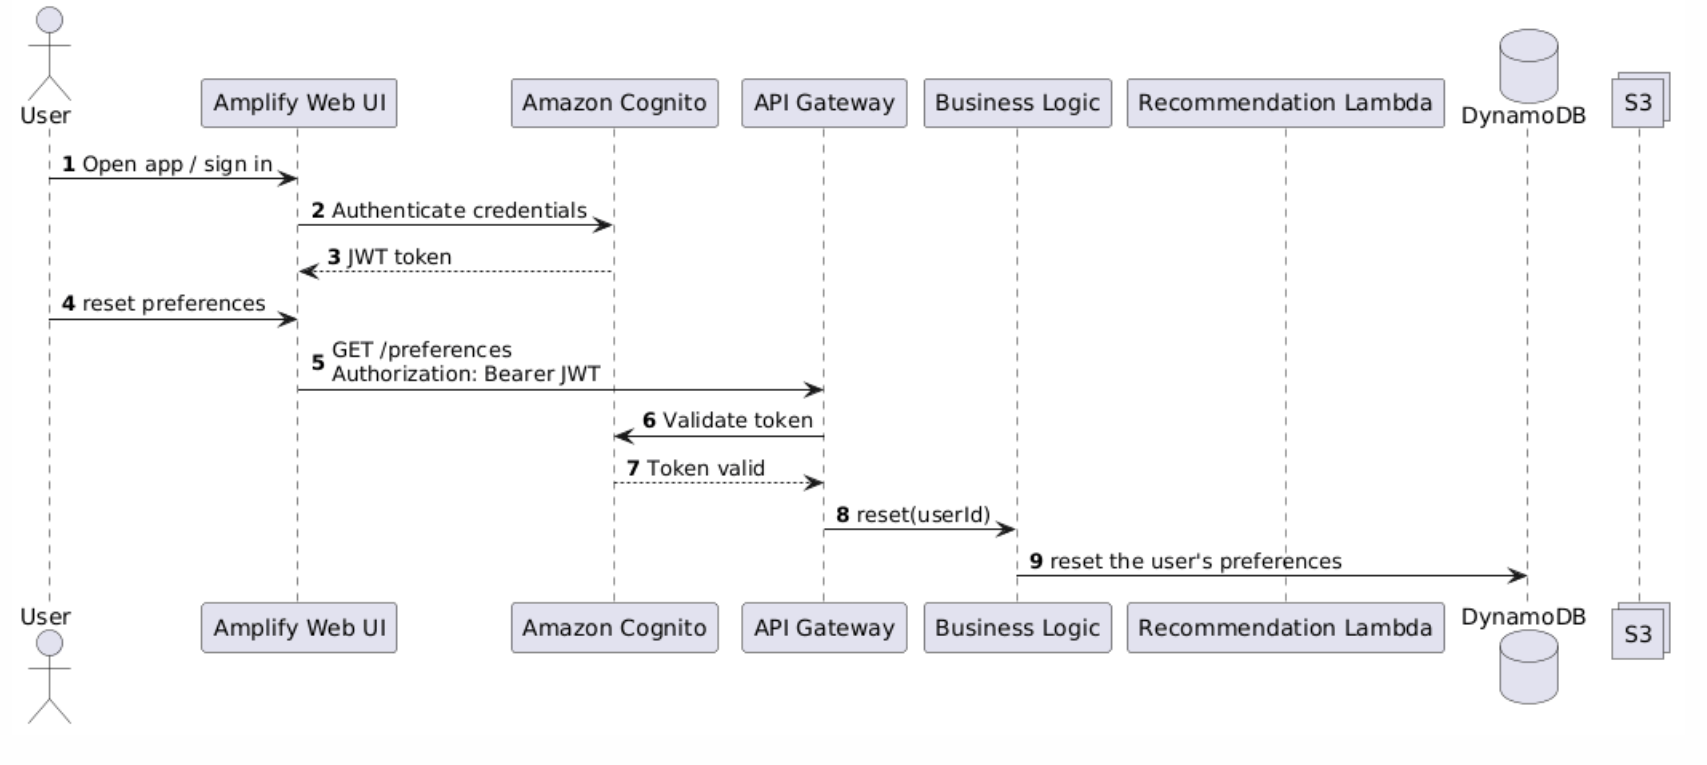
\includegraphics[width=0.9\textwidth]{diagramme_seq_raz.png}
        \caption{Diagramme de séquences de remise à zéros des préférences}
    \end{figure}

    \item \textbf{"Storyboard" du site web}
    \begin{figure}[h]
        \centering
        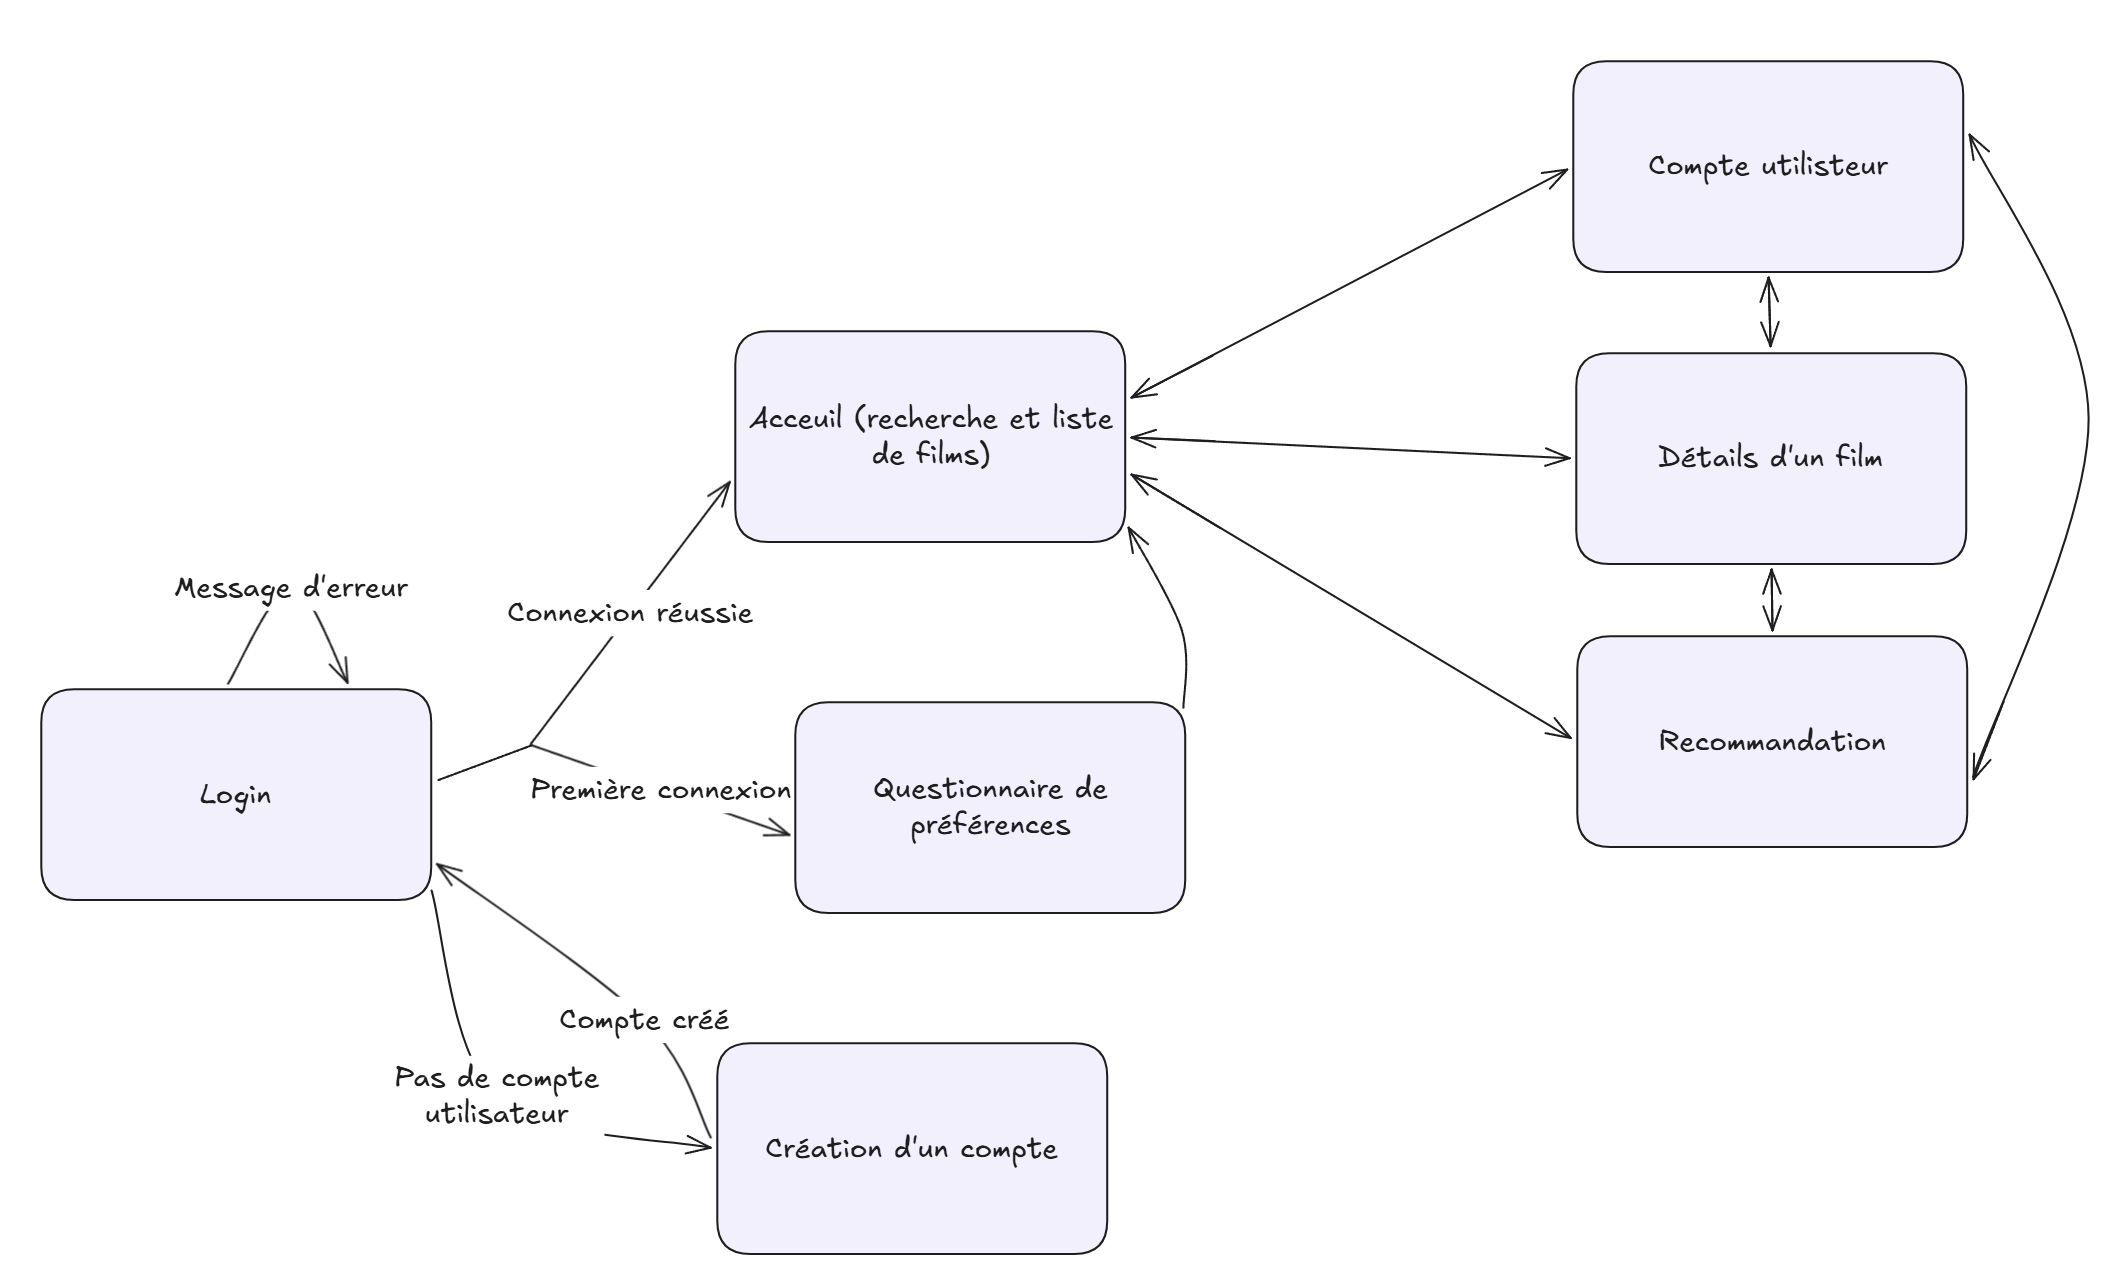
\includegraphics[width=0.98\textwidth]{storyboard.png}
        \caption{Storyboard}
    \end{figure}
\end{itemize}
\newpage

\chapter{Conception détaillée}
\section{Description des modules — Frontend}

\subsection{Interface utilisateur – application Vue.js}
\label{vue}
\subsubsection{Description générale}
Le module d’interface utilisateur constitue la couche de présentation de l’application.\\ Il permet aux utilisateurs d’interagir avec le système de recommandation de films à travers une interface web développée avec Vue.js et déployée via AWS Amplify Hosting.\\
Ce module couvre les interactions principales avec l’application :

\begin{itemize}
    \item Création de compte utilisateur (FR-03).
    \item Authentification et connexion (FR-04).
    \item Formulaire de première connexion (FR-05).
    \item Consultation des films (FR-08). 
    \item Recherche de films (FR-09). 
    \item Notation des films (FR-07).
    \item Affichage des recommandations personnalisées (FR-06).

\end{itemize}
    L’interface communique avec les services backend via AWS AppSync (GraphQL) pour l’accès données et Amazon API Gateway (rest) pour l’appel du moteur de recommandation.

\subsubsection{Composants utilisés / utilisateurs}
\textbf{Utilise :} 
\begin{itemize}
    \item AWS Amplify Auth pour l’authentification via Amazon Cognito.
    \item AWS AppSync (GraphQL) pour accéder aux données stockées dans DynamoDB.
    \item Amazon API Gateway pour appeler la fonction Lambda de recommandation.
    \item Vue Router pour la gestion de la navigation entre les pages.
    \item Tailwind CSS pour la mise en forme de l’interface utilisateur.
    \item FontAwesome pour l’utilisation d’icônes dans l’interface.
\end{itemize}
\textbf{Utilisé par:} 
\begin{itemize}
    \item Les utilisateurs de l'application via un navigateur web.
\end{itemize}

\subsubsection{Interface avec le backend}
La communication entre le frontend et le backend s’effectue via des requêtes HTTPS sécurisées.\\
Deux types d'API sont utilisées :

\textbf{API GraphQL - AWS AppSync}\\
Les principales opération utilisées:
\begin{itemize}
    \item Récupération des films.
    \item Recherche de film.
    \item Gestion des préférences utilisateur.
    \item Sauvegarde des notes.
    \item Récupération du profil utilisateur.
\end{itemize}
Exemples d'opérations :
\begin{itemize}
    \item getMovie(movieId)
    \item listMovies(limit,nextToken)
    \item searchMovies(keyword)
    \item saveRating(userId)
\end{itemize}

\textbf{API Rest – Amazon API Gateway}\\
Un endpoint REST est utilisé pour récupérer les recommandations personnalisées.\\
Endpoint: GET /recommendations\\
Entrée: Token JWT cognito transmis dans le header HTTP.\\
Sortie: Liste d’au moins 6 films recommandés.\\

\subsection{Module de navigation - Vue Router}
\label{vr}
\subsubsection{Description générale}
La navigation entre les pages de l’application est gérée par la bibliothèque Vue Router.\\
Ce module permet de définir les différentes routes correspondant aux vues de l’interface et d’assurer une navigation fluide sans rechargement complet de la page.\\
Certaines routes sont protégées et nécessitent que l’utilisateur soit authentifié avant d’y accéder.\\
\textbf{Routes principales:}
\begin{table}[htbp]
    \centering
    \begin{tabular}{c|c|p{8cm}}
    \hline
    \textbf{Route} & \textbf{Composant Vue} & \textbf{Description} \\ \hline
    /login & LoginPage.vue & Page de connexion \\ \hline
    /register & RegisterPage.vue & Page de création de compte \\ \hline
    /profile & ProfilePage.vue & Page de profil et informations sur les données enregistrées du formulaire de première connexion \\ \hline
    /movie & MoviePage.vue & Page d’affichage de la liste des films et de recherche \\ \hline
    /movie/ :id & MovieDetailsPage.vue & Affichage des détails d’un film \\ \hline
    /form & FormPage.vue & Page du formulaire de première connexion \\ \hline
    \end{tabular}
    \caption{Les routes principales de l'application Vue.js}
\end{table}

\subsection{Module Composants Vue}
\label{cv}
\subsubsection{Description générale}
L’interface est composée de plusieurs composants Vue réutilisables permettant de structurer l’affichage et de faciliter la maintenance du code.\\
Ces composant sont utilisés dans les différentes vues de l’application.\\
\textbf{Composants principaux:}\\

\begin{table}[h]
    \centering
    \begin{tabular}{c|c}
    \hline
    Composant & Rôle \\ \hline
    Navbar.vue & Barre de navigation  \\ \hline
    MovieCard.vue & Affichage d’un film \\ \hline
    RatingComponent.vue & Système de notation \\ \hline
    SearchBar.vue & Barre de recherche \\ \hline
    RecommendationList.vue & Affichage des films recommandés \\ \hline
                     
    \end{tabular}
    \caption{Les composants principaux de l'interface utilisateur}
\end{table}
Ces composants permettent de séparer la logique de présentation et d’assurer une meilleure réutilisation du code.

\subsection{Module Communication API}
\label{ts}
Le module communication API assure l'échange de données entre l'interface web et les services backend de l'application.\\
Il centralise les appels aux différents services AWS afin de séparer la logique de communication réseau de la logique d'interface utilisateur.\\
Ce module utilise le cadre que propose AWS Amplify afin de faciliter l'intégration entre l'application frontend développée en Vue.js et TypeScript et les services backend tel que AWS AppSync et Amazon API Gateway.\\
La centralisation des appels API permet d'améliorer la maintenabilité du code et de simplifier l'utilisation des données dans les différents composants de l'interface utilisateur.\\

\subsubsection{Composants utilisés / utilisateurs}
\textbf{Utilise:}
\begin{itemize}
    \item AWS Amplify API pour la communication avec les services backend.
    \item AWS AppSync (GraphQL) accéder aux données stockées dans DynamoDB.
    \item Amazon API Gateway (REST) pour l'appel du moteur de recommandation.
    \item TypeScript pour le typage des données échangées entre le frontend et le backend.
\end{itemize}
\textbf{Utilisé par:}
\begin{itemize}
    \item Les différents composants Vue de l'application.
    \item Les vues principales de l'interface utilisateur (films, recherche, recommandations).
\end{itemize}

\newpage
\textbf{Services principaux:}
\begin{table}[h]
    \centering
    \begin{tabular}{c|c}
        \hline
        \textbf{Service}   & \textbf{Rôle} \\ \hline
        auth.ts  & gestion de l'authentification avec Amazon Cognito \\ \hline
        api.ts  & communication avec l'API GraphQL AWS AppSync \\ \hline
        recommendation.ts  & appel de l'endpoint REST /recommendation \\ \hline
    \end{tabular}
    \caption{Les services utilisés pour la communication avec les API}
\end{table}

Ces services permettent d'isoler les appels aux API et de faciliter leur utilisation dans les composants Vue.

\section{Description des modules — Backend}

\subsection{Module Authentification — AWS Cognito (Amplify Auth)}
\label{cogn}

\subsubsection{Description générale}

Ce module couvre la création de compte (FR-03) et l'authentification (FR-04). Il est entièrement géré par AWS Cognito via Amplify Auth : l'équipe configure le service dans \texttt{amplify/auth/resource.ts} sans écrire de logique d'authentification. Cognito génère les tokens JWT utilisés par AppSync pour identifier l'utilisateur sur chaque requête GraphQL.

\subsubsection{Composants utilisés / utilisateurs}

\textbf{Utilise :} service AWS Cognito (User Pool), Amplify Auth (configuration déclarative TypeScript).

\textbf{Utilisé par :}
\begin{itemize}
\item AWS AppSync (vérifie le token JWT pour les requêtes GraphQL)
\item Amazon API Gateway (vérifie le token JWT pour \texttt{GET /recommendations})
\item Module Lambda de recommandation (récupère le \texttt{userId} depuis le contexte de la requête)
\end{itemize}

\subsubsection{Attributs Cognito générés automatiquement}

\begin{table}[htbp]
\centering
\begin{tabular}{lp{10cm}}
\toprule
\textbf{Attribut} & \textbf{Rôle} \\
\midrule

sub (userId) & Identifiant unique de l'utilisateur généré par Cognito. Il sert de clé principale dans toutes les collections DynamoDB du projet. \\

email & Adresse email de l'utilisateur utilisée comme identifiant de connexion (\texttt{loginWith: email}). \\

email\_verified & Booléen indiquant si l'adresse email a été confirmée par l'utilisateur après réception du code de vérification. \\

custom:username & Nom d'utilisateur affiché dans l'interface de l'application (attribut personnalisé optionnel). \\

\bottomrule
\end{tabular}
\caption{Attributs utilisateur générés par Amazon Cognito}
\end{table}
\newpage
\textbf{Flux d'inscription :}

\begin{enumerate}
\item L'utilisateur saisit son email et son mot de passe dans l'application Vue.js
\item Amplify Auth appelle le service AWS Cognito
\item Cognito envoie un email contenant un code de vérification
\item L'utilisateur saisit le code reçu
\item Le compte est activé
\end{enumerate}

 
\subsection{Module Schéma de données — Amazon DynamoDB}
\label{dyna}
\subsubsection{Description générale}

DynamoDB est la base de données NoSQL du projet, configurée via Amplify Data. Elle stocke toutes les données métier. Chaque collection utilise le \textit{sub} Cognito (userId) comme clé de partition pour les données personnelles. DynamoDB n'est pas une base de données relationnel : il n'y a pas de jointures, les données sont conçues pour répondre efficacement aux accès les plus fréquents.

\subsubsection{Collection Movie}

Contient les films importés depuis \textit{The Movies Dataset}. Cette collection est en lecture seule depuis l'application et est importée une seule fois lors de l'initialisation du système.

\begin{table}[htbp]
\centering
\begin{tabular}{llp{8cm}}
\toprule
\textbf{Attribut (clé DynamoDB)} & \textbf{Type} & \textbf{Description} \\
\midrule
movieId (PK) & String & Identifiant unique du film (tmdbId). Clé de partition. \\

title & String & Titre du film. \\

overview & String & Résumé du film. \\

genres & List & Liste des genres (ex. : ["Action", "Drama"]). \\

keywords & List & Liste des mots-clés de film. Utilisée par l'algorithme TF-IDF. \\

releaseDate & String & Date de sortie du film (format YYYY-MM-DD). \\

voteAverage & Number & Note moyenne issue du dataset (0 à 10). \\

voteCount & Number & Nombre de votes présents dans le dataset. \\

director & String & Nom du réalisateur extrait de credits.csv. \\

posterPath & String & Chemin de l'affiche (URL base TMDB). \\

\bottomrule
\end{tabular}
\caption{Schéma de la collection Movie}
\end{table}

\newpage

\subsubsection{Collection Rating}

Stocke les notes attribuées par les utilisateurs aux films (FR-07). Une clé composite (userId + movieId) est utilisée afin de garantir l'unicité de chaque notation.

\begin{table}[htbp]
\centering
\begin{tabular}{llp{8cm}}
\toprule
\textbf{Attribut (clé DynamoDB)} & \textbf{Type} & \textbf{Description} \\
\midrule
userId (PK) & String & Identifiant Cognito (sub). Clé de partition. \\

movieId (SK) & String & Identifiant du film. Clé de tri permettant de récupérer toutes les notes d'un utilisateur en une seule requête. \\

rating & Number & Note attribuée par l'utilisateur (0.5 à 5.0 par pas de 0.5). \\

isInitial & Boolean & True si la note provient du questionnaire initial (FR-05). Permet la remise à zéro sélective. \\

createdAt & String & Date de création de la note (format ISO 8601). \\

updatedAt & String & Date de dernière modification. \\

\bottomrule
\end{tabular}

\caption{Schéma de la collection Rating}
\end{table}

\subsubsection{Collection Preference}

Stocke les genres favoris sélectionnés lors du questionnaire initial (FR-05). Ces données servent d'amorce pour l'algorithme de recommandation lorsque l'utilisateur n'a pas encore attribué de notes.

\begin{table}[htbp]
\centering
\begin{tabular}{llp{8cm}}
\toprule
\textbf{Attribut (clé DynamoDB)} & \textbf{Type} & \textbf{Description} \\
\midrule
userId (PK) & String & Identifiant Cognito (sub). Clé de partition. \\

genres & List & Liste des genres sélectionnés (ex. : ["Action", "Comedy"]). \\

hasCompleted & Boolean & True si le questionnaire initial a été complété. Utilisé par le frontend pour contrôler l'affichage du questionnaire. \\

createdAt & String & Date de création de l'enregistrement. \\

\bottomrule
\end{tabular}
\caption{Schéma de la collection Preference}
\end{table}
\newpage
\subsubsection{Collection UserProfile}

Stocke les informations complémentaires du profil utilisateur qui ne sont pas gérées directement par Amazon Cognito.

\begin{table}[htbp]
\centering
\begin{tabular}{llp{8cm}}
\toprule
\textbf{Attribut (clé DynamoDB)} & \textbf{Type} & \textbf{Description} \\
\midrule
userId (PK) & String & Identifiant Cognito (sub). Clé de partition. \\

username & String & Nom d'utilisateur affiché dans l'interface de l'application. \\

createdAt & String & Date de création du profil utilisateur. \\

\bottomrule
\end{tabular}
\caption{Schéma de la collection UserProfile}
\end{table}
\newpage

\subsection{Module Couche API — AppSync (GraphQL) + API Gateway (REST)}
\label{api}
\subsubsection{Description générale}

La couche API combine deux services complémentaires. AWS AppSync expose une API GraphQL qui gère toutes les opérations CRUD courantes : films, notes, préférences et profil utilisateur. AppSync génère automatiquement les résolveurs DynamoDB via Amplify. Amazon API Gateway expose un endpoint REST (\texttt{GET /recommendations}) qui déclenche la fonction Lambda Python de recommandation. Les deux services authentifient chaque requête via le token JWT Cognito.

\subsubsection{Composants utilisés / utilisateurs}

\textbf{Utilise :} collections DynamoDB (Movie, Rating, Preference, UserProfile), fonction Lambda Python (Module 4.4 — via API Gateway uniquement), Amazon Cognito (vérification JWT).

\textbf{Utilisé par :} frontend Vue.js via le client Amplify généré automatiquement.

\subsubsection{Règles d'autorisation}

La règle \texttt{allow.owner()} dans le schéma Amplify garantit qu'un utilisateur ne peut lire et modifier que ses propres données. Les films sont accessibles en lecture à tous les utilisateurs authentifiés.
\newpage
\subsubsection{Opérations exposées — AppSync (GraphQL) et API Gateway (REST)}


\begin{table}[htbp]
\centering
\begin{tabular}{p{3cm} p{3cm} p{2cm} p{3.5cm} p{4cm}}
\toprule
\textbf{Opération} & \textbf{Service} & \textbf{Type} & \textbf{Entrée} & \textbf{Retour} \\
\midrule

createUserProfile & AppSync \newline (GraphQL) & Mutation & username & Profil créé \\

savePreferences & AppSync \newline(GraphQL) & Mutation & userId, genres[] & Préférences enregistrées \\

resetPreferences & AppSync \newline(GraphQL) & Mutation & userId & Préférences supprimées \\

saveRating & AppSync \newline (GraphQL) & Mutation & userId, movieId, rating (0.5--5.0) & Note enregistrée \\

deleteRating & AppSync \newline(GraphQL) & Mutation & userId, movieId & Note supprimée \\

getUserProfile & AppSync\newline (GraphQL) & Query & userId & Profil utilisateur \\

getPreferences & AppSync \newline(GraphQL) & Query & userId & Genres préférés, hasCompleted \\

getMovie & AppSync \newline(GraphQL) & Query & movieId & Détails du film \\

listMovies & AppSync \newline(GraphQL) & Query & limit, nextToken & Liste paginée de films \\

searchMovies & AppSync \newline(GraphQL) & Query & keyword & Films correspondants \\

getUserRatings & AppSync \newline(GraphQL) & Query & userId & Notes de l'utilisateur \\

GET /recommendations & API Gateway (REST) & REST GET & JWT (header) & $\geq$ 6 films recommandés \\

\bottomrule
\end{tabular}
\caption{Opérations exposées par la couche API}
\end{table}
\newpage
\subsection{Module Lambda Python — Algorithme de recommandation }
\label{lamb}
\subsubsection{Description générale}
C'est le seul module entièrement codé en Python par l'équipe. La Lambda est déclenchée par Amazon API Gateway lorsque le frontend appelle GET /recommendations. Elle récupère les données de l'utilisateur depuis DynamoDB, calcule la similarité cosinus entre son profil et tous les films, et retourne au minimum 6 films non encore notés. Elle couvre FR-01 et FR-06.
\subsubsection{Composants utilisés/utilisateurs}
\begin{itemize}
    \item Utilise : DynamoDB (collections Rating, Preference, Movie), bibliothèques Python : boto3, numpy, scikit-learn.
    \item Utilisé par : Amazon API Gateway (déclenche la Lambda via endpoint REST GET /recommendations).
\end{itemize}
\subsubsection{Structure des fichiers}

\begin{table}[htbp]
\centering
\begin{tabular}{lp{10cm}}
\toprule
\textbf{Fichier} & \textbf{Rôle} \\
\midrule

\texttt{handler.py} & Point d'entrée de la fonction Lambda. Contient la fonction \texttt{lambda\_handler(event, context)} qui orchestre les appels aux autres modules. \\

\texttt{dynamo\_client.py} & Fonctions d'accès à DynamoDB : lecture des notes utilisateur, préférences et films. \\

\texttt{recommender.py} & Implémentation de l'algorithme de recommandation : construction du profil utilisateur, calcul de similarité cosinus, filtrage et tri des résultats. \\

\texttt{requirements.txt} & Dépendances Python utilisées par la Lambda : \texttt{numpy}, \texttt{scikit-learn}, \texttt{boto3}. \\

\bottomrule
\end{tabular}
\caption{Structure des fichiers du module de recommandation}
\end{table}
\newpage
\subsubsection{Fonctions — dynamo\_client.py}
\label{dynamo}
\begin{table}[htbp]
\centering
\begin{tabular}{lp{3cm}p{3cm}p{6cm}}
\toprule
\textbf{Fonction Python} & \textbf{Paramètres} & \textbf{Retour} & \textbf{Rôle} \\
\midrule

\texttt{get\_user\_ratings()} & user\_id: str & list[dict] & Requête DynamoDB sur la collection Rating (PK=userId). Retourne \texttt{[{movieId, rating}, ...]}. \\

\texttt{get\_user\_preferences()} & user\_id: str & list[str] & Requête DynamoDB sur la collection Preference. Retourne la liste des genres favoris. \\

\texttt{get\_all\_movies()} & — & list[dict] & Scan de la collection Movie. Retourne tous les films avec leur vecteur TF-IDF pré-calculé. \\

\texttt{get\_rated\_movie\_ids()} & user\_id: str & list[str] & Retourne uniquement les \texttt{movieId} déjà notés afin de les exclure des recommandations. \\

\bottomrule
\end{tabular}
\caption{Fonctions d'accès à DynamoDB}
\end{table}
\newpage
\subsubsection{Fonctions — recommender.py}
\label{recom}
\begin{table}[htbp]
\centering
\begin{tabular}{lp{3cm}p{3cm}p{6cm}}
\toprule
\textbf{Fonction Python} & \textbf{Paramètres} & \textbf{Retour} & \textbf{Rôle} \\
\midrule

\texttt{build\_tfidf\_matrix()} & movies: list & matrix, vectorizer, index\_map & Construit la matrice TF-IDF à partir des genres et des mots-clés. Appelée une seule fois lors du pré-traitement du dataset. \\

\texttt{build\_user\_profile()} & ratings: list, movies\_map: dict & \texttt{np.ndarray | None} & Construit le profil utilisateur comme somme pondérée des vecteurs TF-IDF des films notés $\geq$ 3.5. Retourne \texttt{None} si aucune note valide. \\

\texttt{get\_genre\_profile()} & genres: list, movies\_map: dict & np.ndarray | None & Pour une première connexion basée sur les genres favoris remplis dans le formulaire. Retourne \texttt{None} si aucun film correspondant. \\

\texttt{compute\_scores()} & user\_vec, movies\_map: dict & list[dict] & Calcule la similarité cosinus entre le profil utilisateur et chaque film non encore vu. Retourne \texttt{[{film, score}, ...]}. \\

\texttt{get\_recommendations()} & user\_id: str, n: int = 10 & list[dict] & Fonction principale qui orchestre toutes les étapes de l'algorithme de recommandation (voir pseudo-code section 4.4.9). \\

\bottomrule
\end{tabular}
\caption{Fonctions de l'algorithme de recommandation}
\end{table}
\newpage
\subsubsection{Pseudo-code — get\_recommendations()}

\textbf{Rôle :} Fonction orchestratrice appelée par \texttt{lambda\_handler()}. 
Elle coordonne toutes les étapes : récupération des données DynamoDB, choix de la stratégie de profil (notes ou genres), calcul des scores de similarité cosinus, exclusion des films déjà vus, tri et retour du résultat final. 
C'est le point d'entrée de toute la logique de recommandation.

\begin{algorithm}
\caption{get\_recommendations}
\KwIn{user\_id, $n=10$}
\KwOut{Liste de $n$ films recommandés}

\tcp{1. Récupérer les données de l'utilisateur}
ratings $\leftarrow$ get\_user\_ratings(user\_id)\\
preferences $\leftarrow$ get\_user\_preferences(user\_id)\\
movies $\leftarrow$ get\_all\_movies()

\tcp{2. Construire movies\_map pour accès rapide}
movies\_map $\leftarrow \{ film.movieId : film \mid film \in movies \}$

\tcp{3. Construire le profil utilisateur}
\If{ratings n'est pas vide}{
    user\_profile $\leftarrow$ build\_user\_profile(ratings, movies\_map)
}
\Else{
    user\_profile $\leftarrow$ get\_genre\_profile(preferences.genres, movies\_map)
}

\tcp{4. Calculer les scores de similarité}
scores $\leftarrow$ compute\_scores(user\_profile, movies)

\tcp{5. Exclure les films déjà notés}
rated\_ids $\leftarrow$ get\_rated\_movie\_ids(user\_id)

scores $\leftarrow$ scores sans les films dont movieId $\in$ rated\_ids

\tcp{6. Trier et retourner les n meilleurs films}
trier scores par ordre décroissant

\Return les $n$ premiers éléments de scores
\end{algorithm}

\newpage

\subsection{Module Amazon S3 — Stockage des fichiers}
\label{s3}
\subsubsection{Description générale}

Amazon S3 est utilisé comme espace de stockage de fichiers statiques et de données volumineuses qui ne sont pas adaptées à DynamoDB. Il stocke le dataset \textit{The Movies Dataset} importé depuis Kaggle, les posters des films ainsi que les éventuels artefacts du modèle TF-IDF (vecteurs pré-calculés).

Ce module ne nécessite pas de code spécifique écrit par l'équipe : les opérations de lecture et d'écriture sont réalisées via les SDK AWS ou directement via la console AWS.

\subsubsection{Contenu des buckets S3}

\begin{itemize}

\item \textbf{dataset/} — contient les fichiers CSV du dataset \textit{The Movies Dataset} :
\texttt{movies\_metadata.csv}, \texttt{credits.csv}, \texttt{keywords.csv}, \texttt{ratings\_small.csv}.

\item \textbf{posters/} — contient les images des affiches de films (format JPG ou PNG), récupérées via l'API TMDB ou extraites du dataset.

\item \textbf{artifacts/} — contient les vecteurs TF-IDF pré-calculés. Ces fichiers sont optionnels si les vecteurs sont stockés directement dans DynamoDB ; ils peuvent être placés dans S3 pour éviter des limitations de taille.

\end{itemize}

\subsubsection{Composants utilisés / utilisateurs}

\textbf{Utilisé par :}

\begin{itemize}

\item Module Lambda Python de recommandation (lecture des artefacts TF-IDF si ceux-ci sont stockés dans S3)

\item Script de pré-traitement du dataset (écriture du dataset transformé)

\item Application frontend Vue.js (affichage des posters via une URL publique S3)

\end{itemize}
\chapter{Annexes}
\begin{enumerate}[label=A.\arabic*, leftmargin=1.7cm]
    \item Les fonctionnalités obligatoires du produit :
    \begin{enumerate}[label=FR-0\arabic*, leftmargin=0.8cm]
        \item Système de recommandation basique.
        \item Interface web fonctionnelle et interactive.
        \item Création d'un compte utilisateur.
        \item Authentification et connexion de l'utilisateur.
        \item Choix des préférences utilisateur, pour amorcer le moteur de recommandation.
        \item Génération d'une liste de films recommandés. 
        \item Notation des films par l'utilisateur.
        \item Affichage des informations d'un film.
        \item Barre de recherche.
    \end{enumerate}
\end{enumerate}

\chapter*{Glossaire}
\addcontentsline{toc}{chapter}{Glossaire}
\begin{itemize}
    \item \underline{API (Application Programming Interface) :} Interface permettant à deux logiciels de communiquer entre eux. Dans ce projet, AppSync et API Gateway exposent des APIs que Vue.js appelle pour accéder aux données.
    \item \underline{API Gateway :} Service AWS qui crée et gère des endpoints REST. Utilisé pour exposer l’endpoint GET /recommendations qui déclenche la Lambda Python.
    \item \underline{AppSync :} Service AWS qui expose une API GraphQL. Gère automatiquement les opérations CRUD sur DynamoDB à partir du schéma défini dans resource.ts.
    \item \underline{Architecture :} L'architecture d'un système informatique désigne l'organisation générale de ses composants logiciels et matériels ainsi que les interactions entre eux.
    \item \underline{Authentication :} Processus permettant de vérifier l’identité d’un utilisateur, par exemple à l’aide d’un identifiant et d’un mot de passe.
    \item \underline{Authorization :} Processus permettant de déterminer les actions ou ressources auxquelles un utilisateur authentifié peut accéder.
    \item \underline{AWS (Amazon Web Services) :} Plateforme de services cloud d’Amazon. Ce projet utilise plusieurs services AWS : Amplify, Cognito, DynamoDB, AppSync, API Gateway, Lambda et S3.
    \item \underline{AWS Amplify :} Framework AWS qui simplifie le développement d’applications web et mobiles. Il génère automatiquement l’infrastructure backend à partir d’un schéma TypeScript.
    \item \underline{Backend :} Le backend est la partie invisible, qui gère le fonctionnement interne du produit (par exemple : les données).
    \item \underline{Base de données :} Une base de données est un ensemble d’informations organisé de manière à être facilement accessible, géré et mis à jour.
     \item \underline{boto3 :} Bibliothèque Python officielle d’AWS permettant d’interagir avec les services AWS depuis du code Python. Utilisée par la Lambda pour lire les collections DynamoDB.
     \item \underline{Cognito :} Service AWS gérant l’authentification et les comptes utilisateurs. Il gère l’inscription, la connexion et génère les tokens JWT.
     \item \underline{CRUD :} Acronyme des quatre opérations de base sur une base de données : Create (créer), Read (lire), Update (modifier), Delete (supprimer).
     \item \underline{Diagramme de séquences :} Un diagramme de séquences est un type de diagramme UML qui représente l’ordre chronologique des interactions entre différents composants d’un système. Il montre comment les objets ou services échangent des messages au cours d’un scénario spécifique.
    \item \underline{Diagramme UML :} Un diagramme UML (Unified Modeling Language) est une représentation graphique utilisée pour modéliser et documenter la structure ou le comportement d’un système logiciel.
    \item \underline{DynamoDB :} Base de données NoSQL d’AWS. Stocke les données du projet : films, notes, préférences et profils utilisateurs sous forme de collections.
    \item \underline{Endpoint :} URL précise exposée par une API pour recevoir des requêtes. Exemple : GET /recommendations est un endpoint d’API Gateway.
    \item \underline{Framework :} Un framework est une structure prête à être utilisée pour développer un logiciel, il contient des outils et des bibliothèques.
    \item \underline{Frontend :} Le frontend est la partie visible du site web, c’est ce avec quoi l’utilisateur interagit directement.
    \item \underline{GraphQL :} Langage de requête pour les APIs permettant au client de demander exactement les champs dont il a besoin. Utilisé par AppSync dans ce projet.
     \item \underline{Interface web :} Une interface web est une interface à laquelle on accède et qui s’affiche grâce à un navigateur web, qui permet un dialogue entre l’utilisateur et le système.
    \item \underline{JWT token :} Un JWT (JSON Web Token) est un format de jeton utilisé pour transmettre des informations de manière sécurisée entre deux parties. Il est souvent utilisé dans les systèmes d’authentification pour représenter l’identité d’un utilisateur après sa connexion et permettre l’accès aux ressources protégées.
    \item \underline{Keywords :} Mots-clés associés à chaque film dans le dataset (fichier keywords.csv). Concaténés avec les genres pour construire le vecteur TF-IDF de chaque film.
    \item \underline{Lambda :} Service AWS permettant d’exécuter du code sans gérer de serveur. Dans ce projet, une Lambda Python calcule les recommandations TF-IDF.
    \item \underline{Mutation :} Opération GraphQL qui modifie des données (créer, modifier, supprimer). Équivalent d’un POST/PUT/DELETE en REST.
    \item \underline{NoSQL :} Type de base de données qui ne suit pas le modèle relationnel classique. Les données y sont stockées sous des formats flexibles comme clé-valeur ou document. DynamoDB est une base de données NoSQL.
    \item \underline{np.ndarray :} Type de données NumPy représentant un tableau de nombres. Utilisé pour stocker les vecteurs TF-IDF des films et le profil mathématique de l’utilisateur.
    \item \underline{NumPy :} Bibliothèque Python spécialisée dans les calculs mathématiques sur des tableaux de nombres. Utilisée pour calculer la similarité cosinus entre vecteurs.
    \item \underline{Query :} Opération GraphQL qui lit des données sans les modifier. Équivalent d’un GET en REST.
    \item \underline{REST (Representational State Transfer) :} Style d’architecture pour les APIs utilisant des URLs et des méthodes HTTP (GET, POST…). API Gateway expose une API REST dans ce projet.
    \item \underline{Résolveur :} Code qui traduit une opération GraphQL en action concrète sur la base de données. Amplify génère automatiquement les résolveurs DynamoDB à partir du schéma.
    \item \underline{S3 (Simple Storage Service) :} Service de stockage de fichiers AWS. Utilisé pour stocker le dataset The Movies Dataset, les posters de films et les artifacts TF-IDF.
    \item \underline{SDK (Software Development Kit) :} Boîte à outils permettant d’utiliser un service depuis un langage de programmation. boto3 est le SDK Python d’AWS.
    \item \underline{Similarité cosinus :} Mesure mathématique calculant la ressemblance entre deux vecteurs. Retourne un score entre 0 (aucune ressemblance) et 1 (identiques). Utilisée pour comparer le profil utilisateur avec les films.
    \item \underline{Stockage d'objet :} Le stockage d'objets consiste à traiter chaque donnée comme un objet individuel, plutôt que comme un bloc ou un fichier faisant partie d'un système de fichiers hiérarchique.
    \item \underline{Système de recommandation :} Un système de recommandation est un système qui permet de proposer des contenus ou des produits en fonction de ses préférences.
    \item \underline{TF-IDF (Term Frequency – Inverse Document Frequency) :} Algorithme qui transforme du texte en vecteur numérique en pondérant l’importance de chaque mot. Utilisé pour représenter les films à partir de leurs genres et keywords.
    \item \underline{TfidfVectorizer :} Classe Python de la bibliothèque scikit-learn qui applique l’algorithme TF-IDF sur du texte et retourne des vecteurs np.ndarray.
    \item \underline{Vue.js :} Framework JavaScript utilisé pour le frontend de l’application. Il communique avec AppSync (GraphQL) et API Gateway (REST).

\end{itemize}

\chapter*{Références}
\addcontentsline{toc}{chapter}{Références}
\begin{itemize}
    \item Rounak,  Banik. « The Movies Dataset ». 2018,\\ \url{https://www.kaggle.com/datasets/rounakbanik/the-movies-dataset/data?select=credits.csv.}
    \item Fournier-S’niehotta, Raphaël. « Systèmes de recommandation »,\\
    \url{https://cedric.cnam.fr/vertigo/cours/RCP217/docs/RCP217-RecSys1.pdf}

    \item « Amazon Cognito ». Amazon Web Services, Inc.,\\
    \url{https://aws.amazon.com/fr/pm/cognito/}

    \item «Amazon DynamoDB». Amazon Web Services, Inc.,\\
    \url{https://aws.amazon.com/fr/dynamodb/}

    \item «API graphiques sans serveur - AWS AppSync - AWS». Amazon Web Services, Inc.,\\
    \url{https://aws.amazon.com/fr/appsync/}

    \item « Gestion des API - Amazon API Gateway - AWS ». Amazon Web Services, Inc.,\\ \url{https://aws.amazon.com/fr/api-gateway/}

    \item « Fonction sans serveur, FaaS sans serveur - AWS Lambda - AWS ». Amazon Web Services, Inc.,\\
    \url{https://aws.amazon.com/fr/lambda/}

    \item « Amazon S3 – Stockage d’objets dans le cloud – AWS ». Amazon Web Services, Inc.,\\
    \url{https://aws.amazon.com/fr/s3/}

    \item scikit-learn: machine learning in Python — scikit-learn 1.8.0 documentation.\\
    \url{https://scikit-learn.org/stable/}

    \item pandas - Python Data Analysis Library.\\
    \url{https://pandas.pydata.org/}

    \item Vue.Js.\\
    \url{https://vuejs.org/}

    \item Vue Router | The Official Router for Vue.Js.\\
    \url {https://router.vuejs.org/}

    \item Tailwind CSS - Rapidly Build Modern Websites without Ever Leaving Your HTML.\\
    \url {https://tailwindcss.com/}

    \item Classic Icon Pack | Font Awesome.\\
    \url{https://fontawesome.com}

    \item Handbook - The TypeScript Handbook. \\
\url{https://www.typescriptlang.org/docs/handbook/intro.html}
     \item OpenClassrooms. \\
     \url{https://openclassrooms.com/fr/courses/8186936-gerez-un-projet-avec-la-methodologie-cycle-en-v/8303259-debutez-la-phase-de-conception-detaillee}


\end{itemize}

\chapter*{Index}
\addcontentsline{toc}{chapter}{Index}
\begin{itemize}
    \item Amazon S3 \pageref{s3}
    \item Api Gateway  \pageref{api}
     \item AppSync \pageref{api} 
    \item Architecture \pageref{archi}
    \item AWS Cognito \pageref{cogn} 
    \item Composants Vue \pageref{cv}
    \item Diagramme UML \pageref{UML}
    \item Domaines fonctionnels \pageref{df}
    \item DynamoDB \pageref{dyna}
    \item dynamo\_client.py \pageref{dynamo}
    \item Lambda Python \pageref{lamb}
    \item recommender.py \pageref{recom} 
    \item TypeScript \pageref{ts}   
    \item Vue Router \pageref{vr}
    \item Vue.js \pageref{vue}
\end{itemize}

\end{document}